\section{\AssertLang -- the assertion language}
\label{sub:SpecO}

Our assertions language, \AssertLang, supports ``standard'' assertions' as well ``object-capability'' assertions. 
The ``standard'' assertions  include the values of fields, implication, quantification etc, as well as ghost fields; the latter can represent user-defined predicates. 
The ``object capability'' assertions express restrictions of an object's eventual authority on some other object.
We define the meaning of ``standard'' assertions'' in section \ref{sect:semantics:assert:standard}, 
and the meaning of the  ``object-capability'' assertions in  sections \ref{sect:semantics:assert:prtFrom}
and  \ref{sect:semantics:assert:prt}.


\subsection{Syntax of \AssertLang}
The syntax of \AssertLang  is given in Definition \ref{f:chainmail-syntax}.
An assertion may be an expression,   a query of the defining class of
  an object, the usual connectives and quantifiers, along 
with two non-standard assertion forms:
(1) \emph{Internal/external} and (2) \emph{Protection}, inspired by the capabilities literature.
\footnoteSD{TODO say how these relate with capability lit;  compare with 
 OOPSLA.}


\begin{definition}
\label{def:assert:syntax}
Generalized expressions, $\re$, and assertions, $A$, in
\AssertLang are defined as follows:

\label{f:chainmail-syntax}
 \[
\begin{syntax}
\syntaxElement{\re}{}
		{
		\syntaxline
				{{\alpha}}
				{{x}}
				{\re.f}
				{\re.f({\overline{\re}})}
		\endsyntaxline
		}
\endSyntaxElement
\\
\syntaxElement{A}{}
		{
		\syntaxline
				{{\re}}
				{{\re} : C}
				{\neg A}
				{A\ \wedge\ A}
				{A\ \vee\ A}
				{\all{x:C}{A}}
				{\ex{x:C}{A}}
		\endsyntaxline
		}
 		{
 		\syntaxline
				{\internal{{\re}}}
 				{\external{{\re}}}
				{\protectedFrom{{\re}} {{\re}}} 
				 {\inside {{\re}}} 
		\endsyntaxline
		}
\endSyntaxElement\\
\end{syntax}
\]
In the above, we expect that $f$ stands  for a field or a ghost-field. 
\end{definition}

\noindent
\textbf{NOTES}  Addresses may appear in assertions; this allows  assertions like $\alpha.bal > 700$, but note that universal quantification over addresses  (eg $\forall \alpha:C.[A]$) is not supported; however, we obtain the same effect through quantification over variables (eg  $\forall x:C.[A]$).  
Moreover, the specification does not distinguish between fields and ghostfields. For instance, $a.balance$ may, in some modules (eg when each account object has a field representing it balance), be a field lookup, while in others (e.g. when the balance is defined though an entry in a lookup table),  it may involve executing a ghost function. 
As we discuss below,  our universal quantification goes only over reachable objects i.e. does not consider objects that ould ger collected if we had a garbage collector, while other systems, eg Dafny quantify over allocated addresses.\footnoteSD{example where this distinction would matter/}
% \footnoteSD{{\textbf{NOTE for us} It also allows assertions like $a1.passwd \neq a2.passwd$, whereas in the past we would have written as $\exists x,y.[\ a1.passwd=x \wedge  a2.passwd=y \wedge x\neq y\ ]$.}} \footnoteSD{{TODO compare with oopsla }}

\begin{definition}[Satisfaction 
of Assertions by module and  state] 
\label{def:chainmail-semantics-all}
of Assertions by module and  state] 
\label{def:chainmail-semantics}
We define satisfaction of an assertion $A$ by a % program 
state $\sigma$ with 
 module $M$ by cases on the shape of $A$, in definitions \ref{def:chainmail-semantics}, \ref{def:chainmail-protection-from}, and 
 \ref{def:chainmail-protection}
\end{definition}

TODO: say why we split the def into three defs. 

\subsection{Semantics of \AssertLang -- first part}
\label{sect:semantics:assert:standard}

% An illustration of the concept of reachable appears in the next subsection, in Fig. \ref{fig:Relevant}.
We   use the evaluation relation, $\eval{M}{\sigma}{e}{v}$,
which says that the expression $e$ evaluates
to value $v$ in the context of state $\sigma$ and module $M$.
As expressions in \LangOO may be recursively defined, their evaluation 
need not   % may not necessarily 
 terminate. Nevertheless, the logic of $A$ remains classical because recursion is restricted
to expressions, and not generally to assertions.
\footnoteSD{
The semantics of $\hookrightarrow$ {is} unsurprising 
(see {the appendices %of the full paper 
\cite{necessityFull}).}
We have taken this approach from \citeasnoun{FASE}, which also contains a mechanized Coq proof that assertions are classical \cite{coqFASE}. } %Fig.\ref{f:evaluation}).


\begin{definition}[Satisfaction 
of Assertions -- first part] 
\label{def:chainmail-semantics}
We define satisfaction of an assertion $A$ by a % program 
state $\sigma$ with 
 module $M$ as:
\begin{enumerate}
\item
\label{cExpr}
$\satisfiesA{M}{\sigma}{{\re}}$ \ \ \ iff \ \ \  $\eval{M}{\sigma}{{\re}}{\true}$
\item
\label{cClass}
$\satisfiesA{M}{\sigma}{{{\re}} : C}$ \ \ \ iff \ \ \  $\eval{M}{\sigma}{{\re}}{\alpha}\   \wedge \ \class{\alpha} {\sigma}= C$
\item
$\satisfiesA{M}{\sigma}{\neg A}$ \ \ \ iff \ \ \  ${M},{\sigma}\nvDash{A}$
\item
$\satisfiesA{M}{\sigma}{A_1\ \wedge\ A_2}$ \ \ \ iff \ \ \  $\satisfiesA{M}{\sigma}{A_1} \   \wedge \ \satisfiesA{M}{\sigma}{A_2}$
\item
$\satisfiesA{M}{\sigma}{A_1\ \vee\ A_2}$ \ \ \ iff \ \ \  $\satisfiesA{M}{\sigma}{A_1}\   \vee \ \satisfiesA{M}{\sigma}{A_2}$

\item
\label{quant1}
$\satisfiesA{M}{\sigma}{\all{x:C}{A}}$ \ \ \ iff \ \ \  
 {$\forall \alpha.[\ \GRelevant \alpha \sigma \wedge  \satisfiesA {M}{\sigma} {\alpha:C}  \ \Longrightarrow   \ \satisfiesA{M}{\sigma} {A[x/\alpha]}\ ]$.} 

\item
\label{quant2}
$\satisfiesA{M}{\sigma}{\ex{x:C}{A}}$ \ \ \ iff \ \ \  
 {$\exists \alpha.[\ \GRelevant \alpha \sigma \wedge  \satisfiesA {M}{\sigma} {\alpha:C}  \ \wedge \ \satisfiesA{M}{\sigma} {A[x/\alpha]}\ ]$.} 
\item
\label{cInternal}
$\satisfiesA{M}{\sigma}{\internal{{\re}}}$ \ \ \ iff \ \ \   $\satisfiesA{M}{\sigma}{{{\re}} : C} \ \wedge\ \ C \in M$
\item
\label{cExternal}
$\satisfiesA{M}{\sigma}{\external{{\re}}}$ \ \ \ iff \ \ \   $\satisfiesA{M}{\sigma}{{{\re}} : C} \ \wedge \ C \notin M$
\end{enumerate}
\end{definition}

\textbf{Notes:}   $\rightarrow$ is part of \AssertLang syntax, while  $\Longrightarrow$ is used in the meta-lnaguge.
\footnoteSD{{TODO: explain that$x$ is fresh in $\sigma$  means that $x$ is not in the domain of the top frame, nor in the top continuation of $\sigma$.
 Note, the assumption $x$ is fresh in $\sigma$ has to be justified. Barendregt convention? Or say how we rename if $x$ is not free.}}
\footnoteSD{{TODO: say that any assertion $A(e)$ can be understood as a shorthand for $\exists x. [ x=e \wedge A(x)]$. or  $forall x. [ x=e \rightarrow A(x)]$?? For example, the  assertion   ${\internal{e}}$ is a shorthand for $\exists x. [ x=e \wedge {\internal{x}}]$. QUESTION: do we need to talk about $=$ in the assertion language?}}
In most cases, satisfaction of an assertion depends on the state $\sigma$, but 
in some cases it also depends on the module: namely execution of expressions (\ref{cExpr}) might need to look up the definition of ghost fields  in $M$, while 
for internal or external provenance (\ref{cInternal} and \ref{cExternal}) we need to know the classes defined in $M$.




\subsection{Semantics of Assertions - second part:
protecting objects} %an object from another}

\label{sect:protect}

As we already discussed in the introduction\footnoteSD{make sure we do discuss there}, in the object capabilities world \emph{permission}, i.e.,  access  \footnoteSD{cite MarkMiller thesis, and our Permission and Authority revisited} to a capability is a necessary precondition to some effect. Motto "authority implies eventual permission".
In our work, we express this as "lack of eventual permission to the relevant capability implies that the given effect will never take place".
For this, we need the concept of "lack of  eventual permission".  

\sdN{
We define such lack of \sdN{eventual} permission as "protected".  
An object $o$ is \emph{protected  from} another, external, object $o'$, if $o'$ can obtain direct access to   $o$ only if 
$o$ is ``introduced'' to some external object $o'''$ by some internal object $o''$ -- where $o'$ and $o'''$ may be different.  We  use the term ``introduce'' in the Mark Miller sense, whereby $o_1$ is is ``introduced'' to $o_2$ by $o_3$, iff either $o_3$ sends to $o_2$ a message containing $o_1$, 
or $o_2$ made a call to $o_3$, and $o_3$ eventually returns  $o_1$ as the result of the call.
} 

%\sdN{The motivation for protection comes from considering eventual executions, but this condition is less practical. Instead, we can obtain sufficient conditions just by observing the heap. In the definition below, we say that $o$ is protected from $o'$ if the last object on any path from $o'$ to $o$ is internal. 
%}

\begin{definition}[Satisfaction 
of Assertions  -- Protected From] 
\label{def:chainmail-protection-from}
\label{sect:semantics:assert:prtFrom}
-- continuing definitions in \ref{def:chainmail-semantics}:
\begin{enumerate}
\item
\label{cProtected}
 $\satisfiesA{M}{\sigma}{\protectedFrom{{\alpha}} {{\alpha_{o}}}}$  \ \ \ \ iff  \ \ \ \ 
 $\alpha\neq \alpha_0$,
 \ \ \ \  and
  \begin{itemize}
 \item
 $\satisfiesA{M} {\sigma} {\internal{\alpha_0}}$
 \\
 or
 \item
$\forall n\in\mathbb{N}. \forall f_1,...f_n.$
$
[\ \ \interpret{\sigma}{\alpha_{o}.f_1...f_n}=\alpha \ \ \  \Longrightarrow \ \ \ \satisfiesA{M} {\sigma} {\internal{{\interpret{\sigma}{\alpha_{o}.f_1...f_{n-1}}}}}\ \ ]$
\end{itemize}
\item
$\satisfiesA{M}{\sigma}{\protectedFrom{{\re}} {{\re_{o}}}}$  \ \ \ iff \\
  $\exists \alpha, \alpha_{o}. [\  \ \eval{M}{\sigma}{{\re}}{\alpha}\ \wedge \eval{M}{\sigma}{{\re_0}}{\alpha_0} \  \wedge \ 
  \satisfiesA{M}{\sigma}{\protectedFrom{{\alpha}} {{\alpha_{o}}}}
 \ \  ]$
 \end{enumerate}
 \end{definition} 
 
 {\textbf{NOTE}  that while simple expressions, $\re$, as in Def. \ref{def:chainmail-semantics},  may mention ghost fields,   the paths $\alpha.f_1....f_n$ 
 from Def. \ref{def:chainmail-protection-from} may not. %We see that because the latter are interpreted in $\sigma$. That is, $\satisfiesA{M}{\sigma}{{\alpha_o.f_1...f_n}=\alpha}$ is weaker than $\interpret{\sigma}{\alpha_{o}.f_1...f_n}=\alpha$. TODO: write the latter as a lemma}

% \vspace{.5cm}
\footnoteSD{JAMES' comment: If is possible that "we" do not know the complete heap (eg we only know about the green stuff.) how do we know whether an object is protected. The answer is that we do not know that it is protected, but we do know that our code guarnartees poreservation of protectedness.
%Nevertheless, if the objects are "robust" then we can prove that some properties will be preserved. 
}
\footnoteSD{
OLD COMMENTS: ${\inside {\_}}$  is central to thinking about capabilities. For example, the balance of an account whose
  password is  encapsulated/protected?  will not decrease in the next step.
  Often, API implementations contain objects whose capabilities, while  crucial for the implementation, if exposed,
would break the intended guarantees of the API. Such objects need to remain confined - see
such an example in Section \ref{s:examples}. 
}
\footnoteSD{{\textbf{TODO} make the connection with domination}}
\footnoteSD{SD Can we think of a better name than protection? \kjx{encapsulation}\sdN{No, encapsulation not good}}

Figure \ref{fig:ProtectedFrom} illustrates \sdN{relative} protection.  
%The left pane shows the objects that are protected from $o_5$\footnoteSD{QUESTION: should we write $5$ or $o_5$?}, the middle pane shows the objects protected from $o_7$, and the right pane shows the objects protected from $o_2$
We highlight the protected objects in yellow. Thus, all objects except $o_6$ are protected from $o_5$ (left pane);\ all objects expect $o_8$ are protected from $o_7$ (middle pane);\ and all objects except $o_3$, $o_6$, $o_7$, and $o_8$ are protected from $o_2$ (right pane). 


\begin{figure}[htb]
\begin{tabular}{|c|c|c|}
\hline \\
\resizebox{4.5cm}{!}{
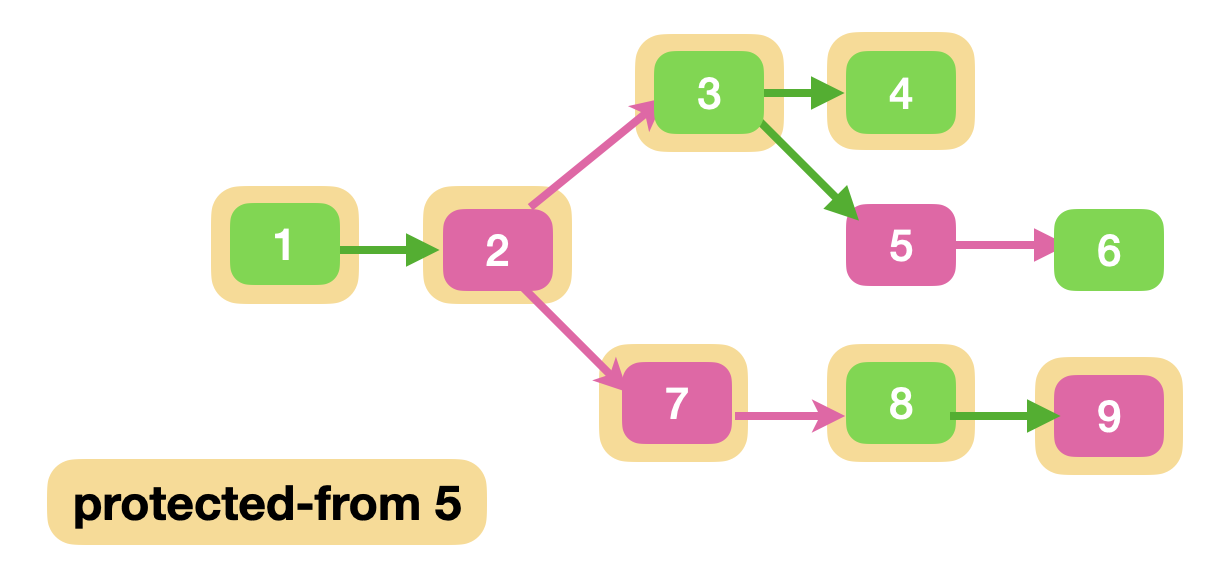
\includegraphics[width=\linewidth]{diagrams/prfA.png}
} 
&
\resizebox{4.5cm}{!}{
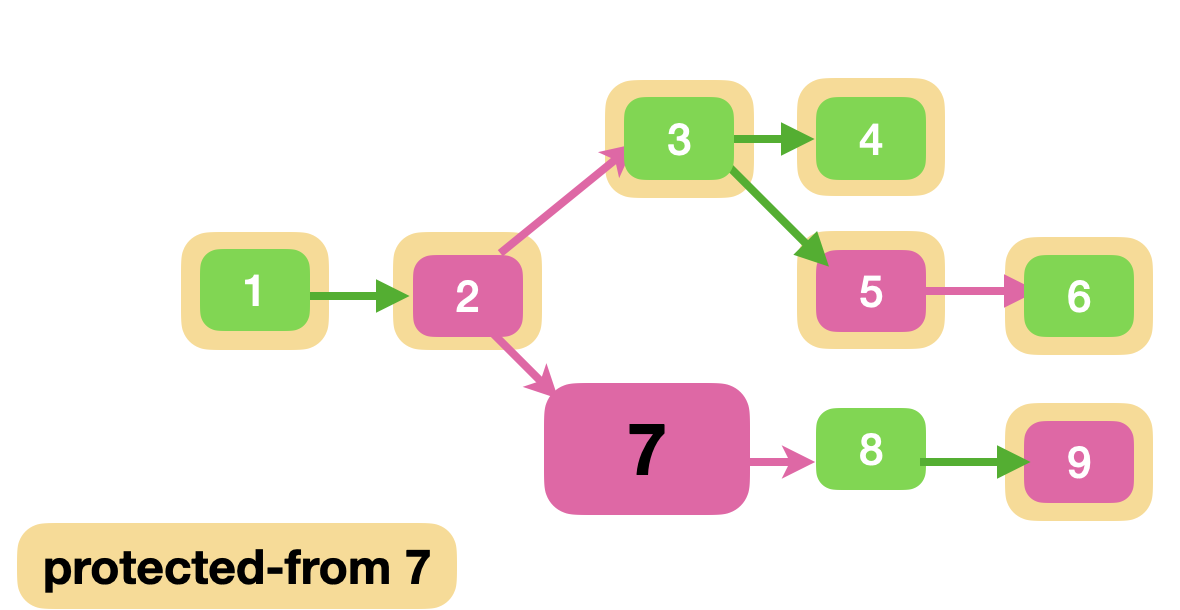
\includegraphics[width=\linewidth]{diagrams/prfB.png}
} 
&
\resizebox{4.5cm}{!}{
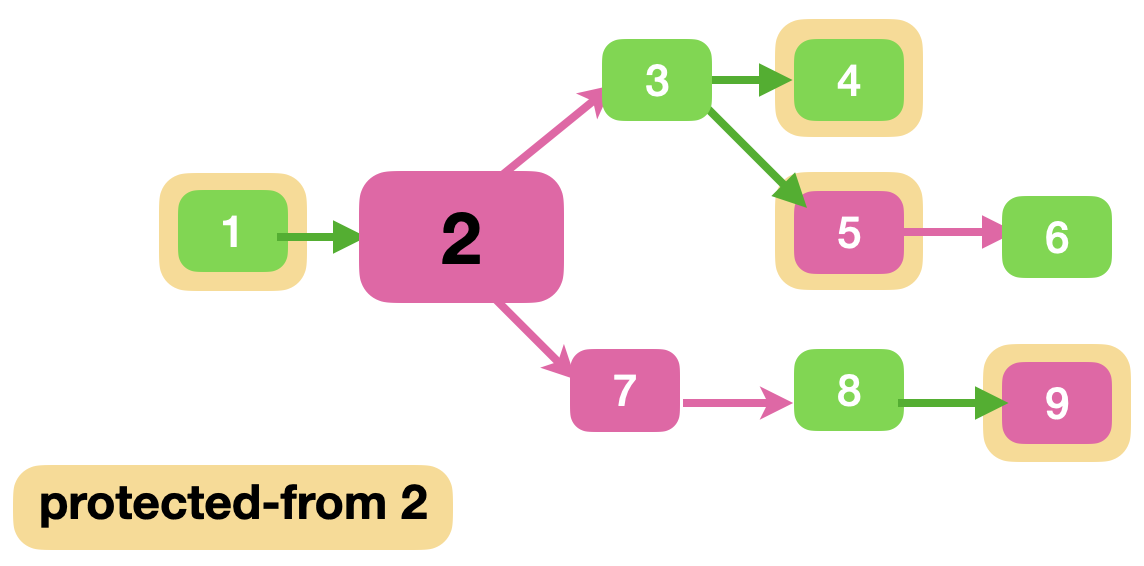
\includegraphics[width=\linewidth]{diagrams/prfC.png}
} 
\\
\hline
protected from $o_5$
&
protected from $o_7$
&
protected from $o_2$
\\
\hline \hline
\end{tabular}
   \caption{Relative Protection. Pink objects are external, and green objects are internal.}
   \label{fig:ProtectedFrom}
 \end{figure}
 
 

Note that $o_8$ is not protected from $o_2$ because there is a path from $o_2$ to $0_8$ which only traverses external objects. Note also, that even though $o_9$ is external, it is protected from $o_7$.
Finally, note that $o_6$ is not protected from $o_2$. 
Namely, even through there are some internal objects on the path from $o_2$ to $o_6$, in our current model, these objects are not sufficient to prevent eventual, unmitigated access of $o_2$ to $o_6$: it is possible for $o_2$ to make a call to $o_3$, and then this call to return $o_5$. Once $o_2$ has access to $o_5$, it can also get access to $o_6$. 

\vspace{.1in}

We now introduce the concept of (absolute) protection.
An object is protected, if it is protected from all locally reachable objects. This could also be understood as 
"an object is protected from the top frame". \footnoteSD{TODO: motivate; many external objects, no matter which one has unprotected access to an object }
 
\begin{definition}[Satisfaction 
of Assertions -- Protected] 
\label{def:chainmail-protection}
\label{sect:semantics:assert:prt}
-- continuing definitions from \ref{def:chainmail-semantics} and \ref{def:chainmail-protection-from}:
\begin{enumerate}
\item
$\satisfiesA{M}{\sigma} {\inside {\re}}$  \ \ \ iff \ \ \ 
\begin{enumerate}
\item
{$\forall \alpha.[ \  \LRelevant {\alpha}  {\sigma}\ \Longrightarrow \ \  \satisfiesA{M}{\sigma}{\protectedFrom{\re} {{\alpha}}}\ ] $}, \ \ \ and 
\item
$\satisfiesA{M}{\sigma}{\external{\prg{this}}}\ \ \Longrightarrow\ \ \forall x\!\in\! \sigma.\ \satisfiesA{M}{\sigma}{x\neq \re}$
\end{enumerate}
\end{enumerate}
\end{definition} 
 
% TODO explain
  Figure \ref{fig:Protected} illustrates %the concept of 
  protection. The heap in all three panes is the same as in  Fig \ref{fig:LReachable} and 
 Fig \ref{fig:ProtectedFrom}. The left pane's  top frame is $\phi_1$; it has  one variable, \prg{this}, pointing to $o_1$.  The middle pane's  top frame is $\phi_2$; it has two  variables,   \prg{this} and \prg{x} pointing to $o_3$ and  $o_7$ resp. The right pane's  top frame is $\phi_3$; it has two  variables,  \prg{this} and \prg{x}, pointing to $o_7$ and$o_3$, resp.  

\begin{figure}[htb]
\begin{tabular}{|c|c|c|}
\hline \\
\resizebox{4.5cm}{!}{
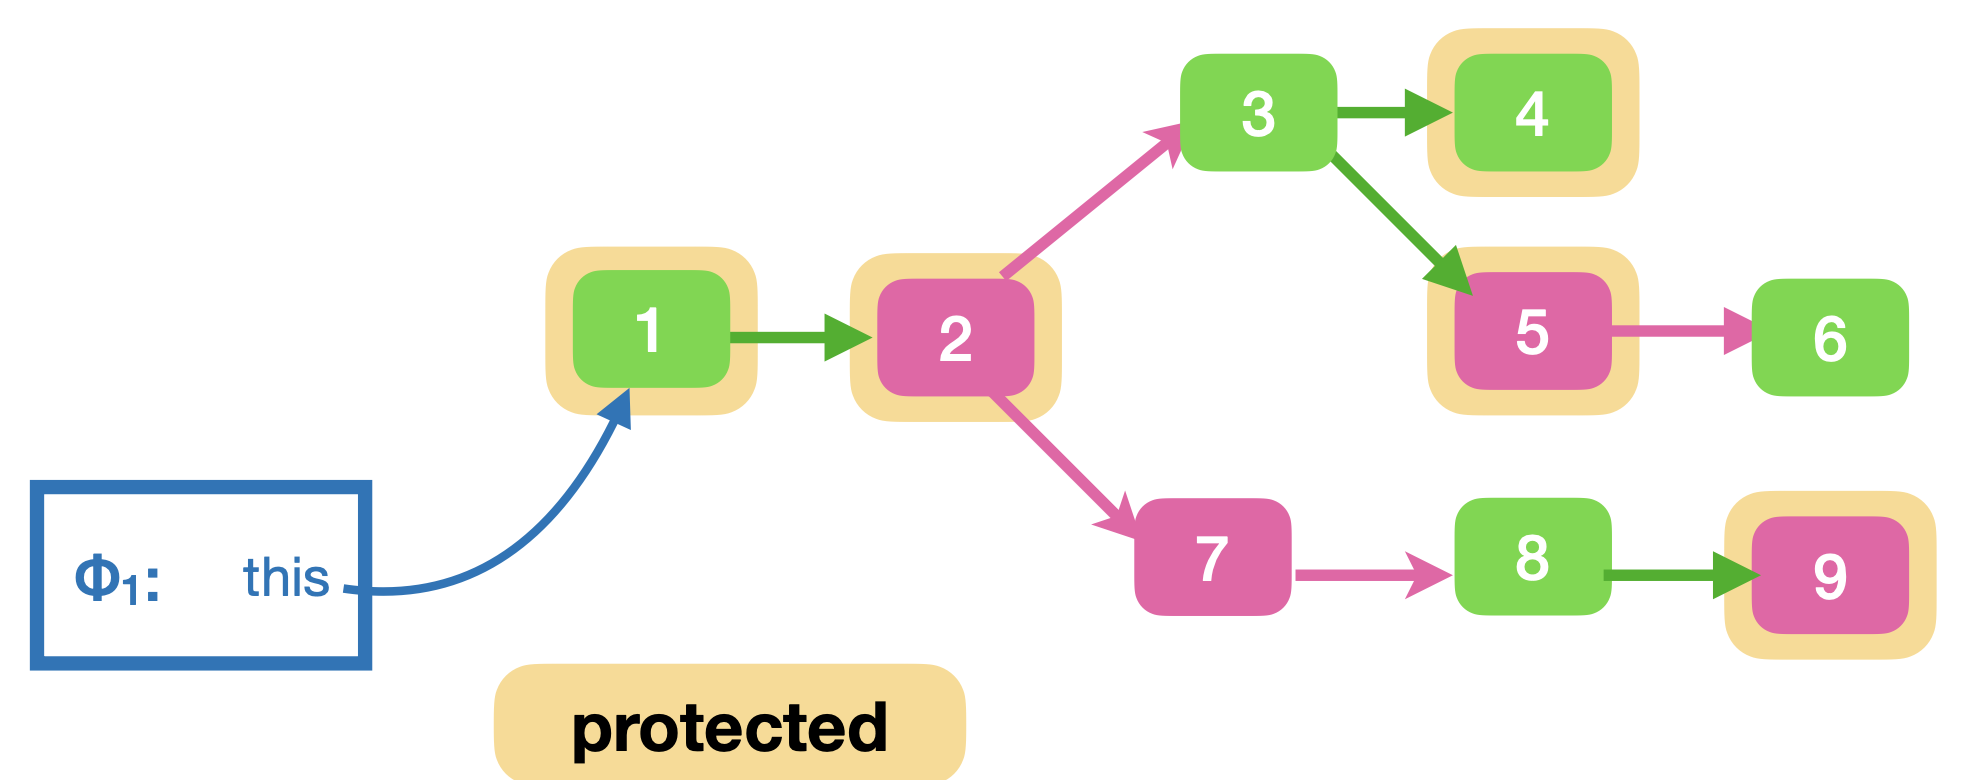
\includegraphics[width=\linewidth]{diagrams/prtFirst.png}
} 
&
\resizebox{4.5cm}{!}{
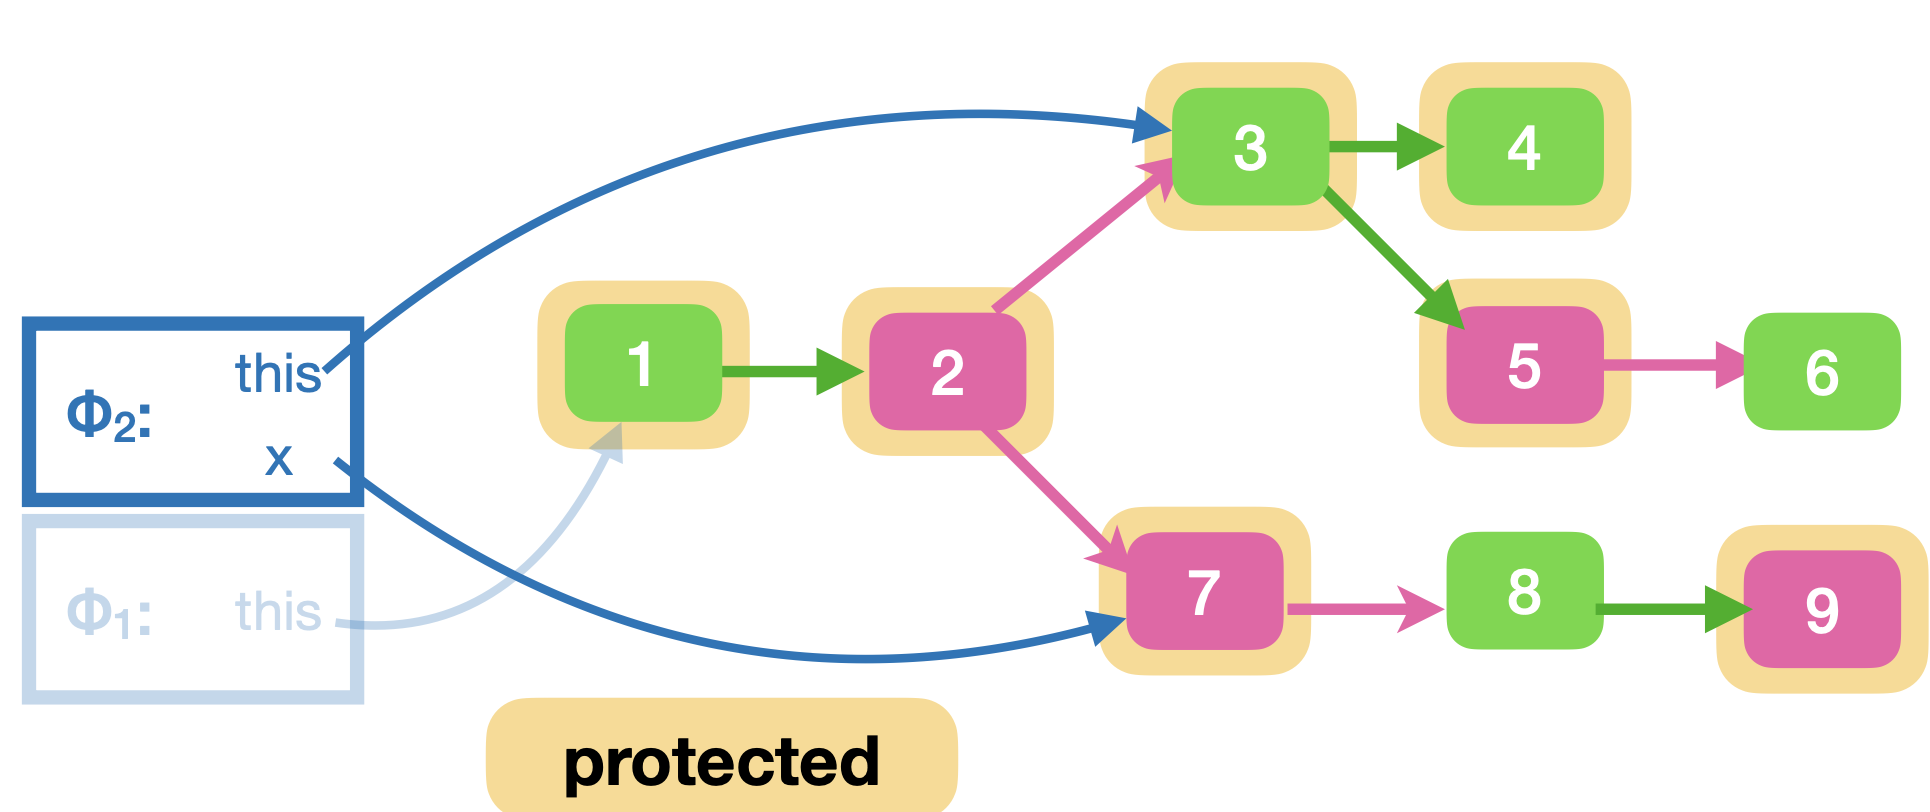
\includegraphics[width=\linewidth]{diagrams/prtSecond.png}
} 
&
\resizebox{4.5cm}{!}{
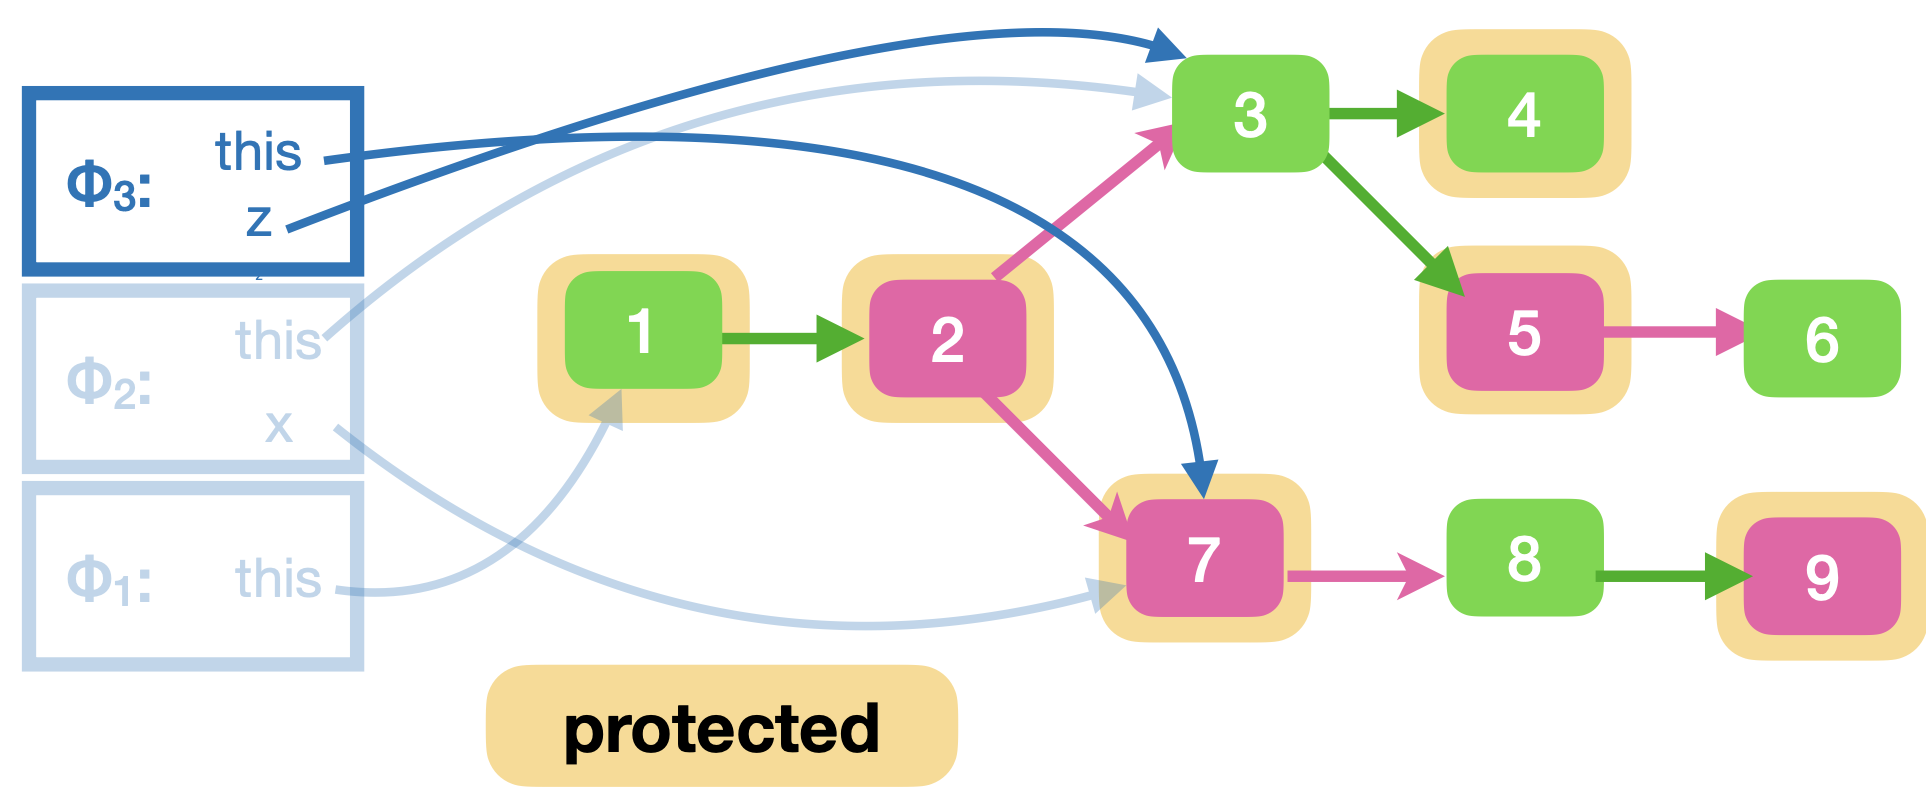
\includegraphics[width=\linewidth]{diagrams/prtLast.png}
} 
\\
\hline
protected  with top frame $\phi_1$ &
protected  with top frame $\phi_2$
&
protected  with top frame $\phi_3$
\\
\hline \hline

\end{tabular}
   \caption{Protected \\
 }
   \label{fig:Protected}
 \end{figure}
 
 
The locally reachable objects from $\phi_1$ were highlighted in the middle pane of.Fig \ref{fig:LReachable}, while the locally reachable object from $\phi_2$ as well as from $\phi_3$ were  highlighted in the right pane of that Figure. 
We highlight the protected objects in each pane with a golden hallo.
 Note that $o_3$ is protected from $\phi_2$, but is not protected from $\phi_3$. This is so, because \prg{this} in $\phi_3$ is external, and  $o_3$ is an argument to the call. That means, that during the call, $o_7$ may obtain unmitigated access (permission?) to $o_3$. 
 
 
   
 \subsection{Viewpoints and Protection}
 
 
\sdN{The examples in Fig. \ref{fig:Protected} demonstrate that validity of assertions which refer to protection may be affected by the pushing and popping of frames on the stack. For example, $o_3$ was not protected with top frame $\phi_1$,   became protected when we pushed the frame $\phi_2$,  and again, is no longer protected when we push $\phi_3$ on the stack. 
The operator $\pushSymbolL$ applies to assertions and sequences of variables: the assertion $\PushAS y A$   guarantees that $A$ will hold after the values if $y$ have been pushed onto a new frame:
 $\PushAS y A$ is \emph{hypothetical}: if a state satisfies $\PushAS y A$, then after pushing
onto that state a frame which contains the values  of $\overline y$, assertion $A$ will hold. }



% Lemma \ref{lemma:vars:to:addresses} says that: (1)Validity of an assertion $A$ in the context of a state $\sigma$ implies  validity of the assertion resulting  from substituting free variables according to the top frame ($A[\sigma]$)}.
%%(2) A bounded execution step (thus not returning from current call)
%in an external state preserves absolute protection.
%(3) An objects which is protected from  the receiver and arguments of a method call, is protected   after the corresponding frame has been pushed onto the stack.

The  push-operator is  defined in Fig. \ref{f:Push}. The only interesting case is the first equation, i.e.  $\PushAS y {(\inside x)}$: For 
$x$ to be protected from the viewpoint of the callee, it should be protected from all the call's arguments, ie from  $\overline y$. That is,
$\protectedFrom x {\overline {y} \ \wedge\ x\neq \overline y}$. 
In all other cases, the operator  $\pushSymbol$  leaves simple assertions unmodified (i.e. the second to sixth equation), or is applied to the sub-assertions (i.e. the seventh to eleventh equation).



\newcommand{\sigmas}{\widetilde \sigma}

 
\begin{figure}[hbt]
$
\begin{array}{c}
\begin{array}{ccc}
  \PushAS y {(\inside x)}\ \triangleq\ \protectedFrom x {\overline {y} }
&\ \  \ \ \ \ \ \ &   \PushAS y {(\protectedFrom x {\overline {u}})}\ \triangleq\ \protectedFrom x  {\overline {u}}  % {(\overline {y'}\setminus \overline {y})} 
\end{array}
  \\
  \\
    \begin{array}{lclclcl}
 \PushAS y  {x:C}\ \triangleq\  x:C 
& &
\PushAS y  {(\internal x)}\ \triangleq\ {\internal x}
& &
\PushAS y  {(\external x)}\ \triangleq\ {\external x}
& &
 \PushAS y  e\ \triangleq\ e
  \end{array}
  \\
  \\
\begin{array}{lclcl}
 \PushAS y   {(A_1  \wedge  A_2)}\ \triangleq\ \PushAS y  { A_1}  \wedge   \PushAS y  {A_2}  & & 
 \PushAS y { (A_1 \vee  A_2)}\ \triangleq\  \PushAS y {A_1}  \vee  \PushAS y {A_2} 
 & &
 \PushAS y  {(\neg A)}\ \triangleq\ \neg( {\PushAS y A} )  
  \\  \\  % \PushAS y  {(\neg A)}\ \triangleq\ \neg( {\PushAS y A} ) & &
 \PushAS y  {(\forall x:C.A)}\ \triangleq\ \forall x:C.({\PushAS y A} )&  &  
  \PushAS y  {(\exists x:C.A)}\ \triangleq\ \exists x:C.({\PushAS y A} )
%\PushAS y  {x:C}\ \triangleq\  x:C 
%& &
%\PushAS y  {(\internal x)}\ \triangleq\ {\internal x}
%& &
%\PushAS y  {(\external x)}\ \triangleq\ {\external x}
\end{array}
\end{array}
$
\caption{The push operator for assertions } 
\label{f:Push}
\end{figure}
 

\vspace{.1cm}

The guarantees given by $\pushSymbolL$ are described in Lemma \ref{lemma:push:ass:state}. (1) If  the current state satisfies  $\PushAS y A$, then the assertion $A$ will hold after pushing a frame with the values of $\overline y$ (here $\PushS {y} {\sigma}$), and after extending the top frame so that all free variables of $A$ point to what they pointed at in the top frame of $\sigma$ (here $[\overline{x \mapsto {\interpret {\sigma} {x}} } ]$). (2) States the opposite: If $A$ holds in a state which is the result of pushing a frame with the values for $\overline y, \overline z$ (here ,
Conversely,   if a state satisfies  $A$ after a top frame containing the  values of $\overline y$  and some other variables has been pushed (here \PushSLong {(\overline y, \overline z)} \sigma), then $\PushAS {y} {A}$ will hold  after popping that frame, and mapping the free variables of $A$ to their values  in the state  before.

\sdN{
\begin{lemma} 
\label{lemma:push:ass:state}
For any states  $\sigma$, $\sigma'$, assertion $A$,  and variables $\overline x$, $\overline y$, $\overline z$ disjoint with one another,  and such that 
$fv(A)\subseteq \overline x$:
\begin{enumerate}
 \item
 \label{lemma:push:ass:state:one}
$M, \sigma \models \PushAS {y} {A}\ \ \ \ \ \ \   \Longrightarrow  \ \ \ \ M,  (\PushS {y} {\sigma})[\overline{x \mapsto {\interpret {\sigma} {x}} } ] \models A$
\item
\label{lemma:push:ass:state:two}
$M, {\PushSLong {(\overline y, \overline z)} \sigma }   \models\  A \  \ \ \ \Longrightarrow  \ \ \ \ M,  \sigma[\overline{x \mapsto {\interpret {\PushSLong {(\overline y, \overline z)} \sigma} {x}} } ] \models  \PushAS  {y} {A}$
\end{enumerate}
\end{lemma}
}


\noindent
\textbf{Notation}  In the above lemma we overloaded the notation: We write $\PushS {y} {\sigma}$ for the set of states that result from pushing a new frame with the values of $\overline y$ onto the stack of $\sigma$.
We lift operators and judgements that apply to one state to apply to sets of states: If  $\sigmas$ is a set of states,  then $\sigmas[ \overline{x \mapsto v}]$ is the set of states from $\sigmas$ to which we applied the substitution. And the   notation 
$M,   \sigmas \models A$ holds if  $M, \  \sigma \models A$ for all $\sigma \in \sigmas$.
  \vspace{.1cm}
  

\vspace{.1cm}
\noindent 
\blue{\textbf{Comment} The $ \pushSymbol$ operator reminds me of the magic wand. Namely, $-\!-\!*$ is spatial and heap based:  the assertion $A -\!-\!* A'$ says: if you combine with a heap that satisfies $A$, then the complete heap will satisfy $A'$. While $\PushASLong {\_} {\_}$ is temporal and  stack based: the assertion  $\PushAS {y} A$ says that if you push a frame with range the values of $\overline y$, then $A$ will hold. \textbf{End Comment} }

%{\red{I am surprised that $ \pushSymbol$  only affects  ${\inside x}$, and leaves all else unmodified,}}


 
